% !TEX root = /home/computer/ucsc/master-2/quarter-2/advanced-fluids/master.tex
\assignment{1}{Tue 04 Jan 2022 15:38}{Assignment 1}

\subsectionfont{\fontsize{12}{12}\selectfont}

% \graphicspath{./assignment_01/figures/}

\section{Mass conservation and other conservation laws}%

\subsection{Mass conservation in polar coordinates}%

\textbf{Question 1}: Express the mass conservation equation in 2D polar
coordinates

mass conservation
\[
  \diffp[]{ \rho}{t} + \nabla \cdot ( \rho \vec{u}) = 0
.\] 

expressed in 2D polar coordinates
\[
  \boxed{\diffp[]{ \rho}{t} + \frac{1}{r} \diffp[]{(r\rho \vec{u}_r)}{r} + \frac{1}{r}
  \diffp[]{( \rho \vec{u}_\theta)}{\theta}= 0}
.\] 

where $\vec{u} = \begin{pmatrix} u_{r} \\ u_{\theta} \end{pmatrix}$ is the
velocity vector field expressed in polar coordinates.


\textbf{Velocity field in polar coordinates} 

Let $ \beta = \{ \vec{v}_r, \vec{v}_\theta\}$ be an orthonormal basis where
\[
\vec{v}_r = \begin{pmatrix} \cos{\theta} \\ \sin{\theta} \end{pmatrix}, \quad
\vec{v}_\theta = \begin{pmatrix} -\sin{\theta} \\ \cos{\theta} \end{pmatrix}.
.\] 

Then at each point $(r,\theta)$ in space
the position of a particle can be expressed as

\[
  \vec{r}(r,\theta) = r\vec{v}_r 
.\] 

\begin{figure}[H]
    \centering
    \incfig{polar}
    \caption{Tangent space? coordinate transform}
    \label{fig:polar}
\end{figure}

 so a fluid particles velocity can be expressed as

 \begin{align*}
   \vec{u}(r, \theta) = \diff[]{[r\vec{v}_r]}{t} &= \diff[]{r}{t}\vec{v}_r+r
   \diffp[]{\vec{v}_r}{ \theta} \diff[]{ \theta}{t}\\
                                                 &= \diff[]{r}{t}\vec{v}_r+r
                                                 \diff[]{ \theta}{t}\vec{v}_{
                                                 \theta} \\
                                                 &= \dot{r} \vec{v}_{r}
                                                 + r \dot{\theta} \vec{v}_{\theta}
 \end{align*}

 then in $ \beta$ (polar) coordinates

 \[
   [\vec{u}(r, \theta)]_{\beta} = \begin{pmatrix}
     \dot{r} \\ r \dot{ \theta} 
   \end{pmatrix}
 .\] 

 \textbf{Question 2}: If $\vec{u} = \begin{pmatrix} u_{r} \\ u_{ \theta}
 \end{pmatrix} = \begin{pmatrix} u_0 \\ 0 \end{pmatrix}$, then a fluid particle
 has speed $u_0$ pointing in the direction of basis vector $\vec{v}_{r}$.

\begin{figure}[H]
    \centering
    \incfig{velocityfield}
    \caption{velocity field}
    \label{fig:velocityfield}
\end{figure}

\textbf{Question 3}: Solve for $ \rho(r,t)$ with initial condition
$ \rho_0(r,t=0) = r e^{-\frac{(r-1)^{2}}{2}}$ and  $\vec{u}_{\beta}
= \begin{pmatrix} u_0 \\ 0 \end{pmatrix}$.

Mass conservation expressed in polar coordinates, and assuming $ \rho$ doesn't
depend on $ \theta$

\[
  \diffp[]{ \rho}{t} + \frac{1}{r} \diffp[]{(r\rho \vec{u}_r)}{r} + \frac{1}{r}
  \diffp[]{( \rho \vec{u}_\theta)}{\theta}= 0
.\] 

becomes

\[
  \diffp[]{ \rho}{t} + \frac{u_0}{r} \diffp[]{(r\rho)}{r} = 0
.\] 

if we let $f(r,t) = r \rho(r,t)$, then we get

\begin{align*}
  \frac{1}{r} \diffp[]{f}{t} + \frac{u_0}{r} \diffp[]{f}{r} &= 0 \\
  \diffp[]{f}{t} + u_0 \diffp[]{f}{r} &= 0
\end{align*}

considering the parameterization $f = f(r(s),t(s)) \implies \diff[]{f}{s}
= \diff[]{t}{s}f_t + \diff[]{r}{s}f_{r} = 0$, we get the following
characteristic equations

\[
\begin{cases}
  \diff[]{t}{s} = 1 & \implies t = s + t_0 \underbrace{\implies}_{t_0 = 0}
  t = s \\
  \diff[]{r}{s} = u_0 & \implies r = u_0s+r_0 \\\\
  \diff[]{f}{s} = 0 & \implies f = f_0(r_0,t_0)
\end{cases}
.\] 

putting everything together
\[
  f(r,t) = f(r_0,t_0=0) = (r-u_0t) \rho_0(r-ru_0t,0) \\
.\] 
\[
  \implies \boxed{\rho(r,t) = (r-u_0t)e^{-\frac{1}{2}(r-u_0t-1)^{2}}}
.\] 

Plotting $ \rho(r,t)$ at various snapshots in time, with $u_0=1$, we see an
agreement with Figure \ref{fig:velocityfield}. The density gets pushed away
from the origin, $r=0$, at a constant speed $u_0$.

\begin{figure}[H]
  \centering
  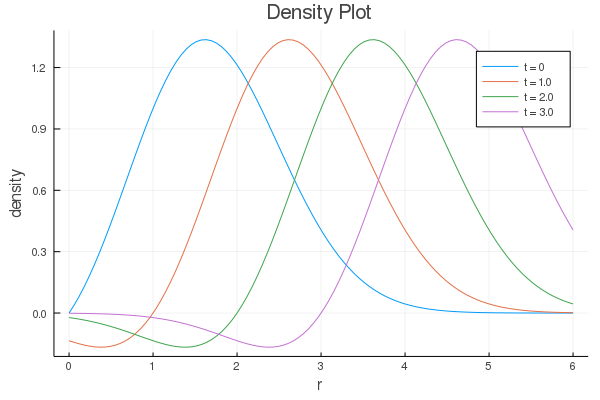
\includegraphics[width=0.8\linewidth]{./assignment_01/figures/plot_q3.png}
  \caption{}%
  \label{fig:plot_q3}
\end{figure}

\subsection{Other conservation laws}%

Assuming $S$ is the salt concentration (mass of salt per unit mass of water) in
salty water. If salt is conserved, then the equation for the evolution of $S$
is the change in salt concentration w.r.t time equal to the (negative)
divergence of salt flux at a point

\[
  \boxed{\diffp[]{S}{t} + \nabla\cdot(S\vec{u}) = 0}
.\] 


\section{Momentum equation and vorticity}%

\textbf{Question 1}: Assuming incompressible flow, and constant kinematic
viscosity $\mu$ is constant, show $\nabla\cdot\Pi = \mu\nabla^{2}\vec{u}$

Since the flow is incompressible $\implies \nabla \cdot \vec{u} = 0$, then the
viscous stress tensor becomes

\begin{align*}
  \Pi &= (k-\frac{2}{3} \mu) \underbrace{ \nabla \cdot \vec{u}}_{=0}I+ \mu
  ( \nabla \vec{u} + ( \nabla \vec{u})^{T}) \\
      &=\mu ( \nabla \vec{u} + ( \nabla \vec{u})^{T}) \\
      &= \mu \left[ \cmatrix{J}{
          \diffp[]{u_1}{x_1} \& \diffp[]{u_1}{x_2} \& \diffp[]{u_1}{x_3} \\
          \diffp[]{u_2}{x_1} \& \diffp[]{u_2}{x_2} \& \diffp[]{u_2}{x_3} \\
          \diffp[]{u_3}{x_1} \& \diffp[]{u_3}{x_2} \& \diffp[]{u_3}{x_3} \\
      } + \ctmatrix{J}\right] \\
      \implies \Pi_{ij} &= \mu \left( \diffp[]{u_{i}}{x_{j}} + \diffp[]{u_{j}}{x_{i}}\right)
\end{align*}

Then the, $i^{\text{th}}$ term of the, divergence of $ \Pi$, for constant kinematic viscosity $ \mu$ 

\begin{align*}
  (\nabla \cdot \Pi)_{i} &= \sum_{j} = \diffp[]{ \Pi_{ji}}{x_{j}} \\
                         &= \mu \sum_{j}\frac{\partial}{\partial x_{j}} \left(
                         \diffp[]{u_{j}}{x_{i}} + \diffp[]{u_{i}}{x_{j}}\right)
                         \\
                         &= \mu\sum_{j} \frac{\partial}{\partial x_{j}} \left(
                         \diffp[]{u_{j}}{x_{i}}\right)
                         + \diffp[2]{u_{i}}{x_{j}} \\
                         &= \mu\sum_{j} \frac{\partial}{\partial x_{i}}
                         \underbrace{\left( \diffp[]{u_{j}}{x_{j}}\right)}_{=
                         \nabla \cdot \vec{u} = 0}
  + \diffp[2]{u_{i}}{x_{j}} & \textbf{equality of mixed partials}\\
                            &= \mu \sum_{j}\diffp[2]{u_{i}}{x_{j}}
\end{align*}

Therefore,
\[
  \boxed{\nabla \cdot \Pi = \mu \nabla^{2} \vec{u}}
.\] 

\textbf{Question 2}: Derive the equation for the evolution of vorticity
$ \omega = \nabla \times \vec{u}$ from the momentum equation 

Assuming density is constant and there is no viscous dissipation $ (\nabla
\cdot\Pi = 0)$, then the momentum equation becomes
\[
  \rho_0 \frac{D\vec{u}}{Dt} = - \nabla p + \underbrace{\nabla
  \cdot\Pi}_{=0}
.\] 

expanding the substantial derivative and multiplying the momentum equation by
$( \nabla\times)$
\[
  \rho_0\left(\nabla\times \left( \diffp[]{\vec{u}}{t} + \vec{u} \cdot
  \nabla\vec{u}\right)\right) = \nabla\times (- \nabla p)
.\] 

by continuity 
\[
  \nabla\times \diffp[]{\vec{u}}{t} = \diffp[]{ (\nabla\times
  \vec{u})}{t} = \diffp[]{ \omega}{t}
.\] 

and using the identity 
\[
(\vec{u} \cdot \nabla)\vec{u}
= (\nabla\vec{u}) \cdot\vec{u} - \vec{u}\times \underbrace{
(\nabla\times\vec{u})}_{= \omega}
.\] 

we have

\[
  \rho_0 \left( \diffp[]{ \omega}{t}
    + \underbrace{\nabla\times[(\nabla\vec{u})}_{=0} \cdot\vec{u} - \vec{u}\times \omega ]\right) = -\underbrace{\nabla\times
\nabla p}_{=0}
.\] 

where the curl of grad is zero $ \nabla\times \nabla ( \cdot) = 0$. Dividing by
$ \rho_0$ 
\[
\diffp[]{ \vec{ \omega}}{t} - \nabla\times\vec{u}\times \vec{ \omega} = 0
.\] 

using the identity $ \nabla\times (\vec{u}\times\vec{ \omega})= \vec{u}
( \underbrace{\nabla \cdot \vec{ \omega}}_{=0}) - \vec{ \omega}
( \underbrace{\nabla \cdot \vec{u}}_{=0})+ (\vec{
\omega} \cdot \nabla)\vec{u}- (\vec{u} \cdot \nabla) \vec{ \omega}$. Where
$ \nabla \cdot \vec{ \omega} = 0$ because it is the divergence of curl, and
$ \nabla \cdot \vec{u} = 0$ due to the flow being incompressible. Therefore,
the equation for the evolution of vorticity is
\[
  \boxed{\diffp[]{\vec{ \omega}}{t} + (\vec{u} \cdot \nabla)\vec{ \omega}
  = (\vec{ \omega} \cdot \nabla)\vec{u}}
.\] 

or, using the substantial derivative

\[
  \boxed{\frac{D\vec{ \omega}}{Dt} =(\vec{ \omega} \cdot \nabla)\vec{u}}
.\] 


\section{Thermal energy equation and hydrostatic equilibrium}%

\subsection{Energy equation}%

Using $\nabla\cdot\Pi=\mu\nabla^{2}\vec{u}$ for incompressible Newtonian fluid,
find the expression for viscous heating $ \phi$

\subsection{Hydrostatics}%
Hydrostatic equilibrium is derived from the momentum equation assuming there is no fluid motion
\[
-\nabla p + \rho \vec{g} = 0
.\] 

\textbf{Question 1}: In Cartesian coordinates with $\vec{g} = -g\vec{e}_{z}$,
we have
\[
- \begin{pmatrix}
  p_{x}\\p_{y}\\p_{z}
\end{pmatrix} = \rho \begin{pmatrix}
  0\\0\\g
\end{pmatrix}
.\] 

\textbf{Question 2}: The liquid equation of state implies density is simply
a function of temperature
\[
  \rho = \rho(T)
.\] 
and since the liquid is isothermal, temperature is constant $T=T_0$. This
implies density is constant
\[
\rho = \rho_0
.\] 

$p_{x}=0 $, and $p_{y}=0$ implies pressure is independent of x and y, so we
have
\[
  p_{z}= - \rho_0g \quad \text{is constant}
.\] 
integrating with respect to $z$ 
\[
  p(z) = -g \rho_0z + p_0 \\
.\] 

since pressure is zero at the surface $p(H) =0\implies p_0= g \rho_0H$, then
pressure increases linearly from $z=H$ to $z=0$
\[
\boxed{p(z) = -g \rho_0z +g \rho_0H}  
.\] 

\begin{figure}[H]
    \centering
    \incfig{pressure1}
    \caption{liquidEOS}
    \label{fig:pressure1}
\end{figure}

\textbf{Question 3}: For an isothermal perfect gas equation of state, pressure
is a function of density only $p( \rho) = R \rho T_0$. So the equation for hydrostatic equilibrium in terms of
density
\[
\rho_{z} = -\rho \frac{g}{RT_0}
.\] 

Integrating with respect to $z$ 
\[
  \ln{ \rho} = - \frac{g}{RT_0}z + c
.\] 
\[
  \implies \boxed{ \rho(z) = \rho_0e^{- \frac{g}{RT_0}z}}
.\] 

Here density decreases exponentially from $z=0$

\begin{figure}[H]
    \centering
    \incfig{perfectgaseos}
    \caption{perfectgasEOS}
    \label{fig:perfectgaseos}
\end{figure}

The scaleheight, $H$, comparing the perfect gas equation of state and Boyles
law

\[
\frac{p}{ \rho} = gmH = RT_0
.\] 





